\documentclass[fleqn, 12pt]{article}
\usepackage[skip=10pt plus1pt, indent=0pt]{parskip}
% --- Packages ---
\usepackage[utf8]{inputenc}
\usepackage{amsmath, amssymb, amsthm} % Math symbols & environments
\setlength{\mathindent}{90pt} % remove default indent
\usepackage{geometry} % Page layout
\geometry{margin=1in}
\usepackage{graphicx} % For figures
\graphicspath{{images/}}
\usepackage{hyperref} % Clickable references
\usepackage{enumitem} % Better lists

% --- Theorem environments ---
\newtheorem{theorem}{Theorem}
\newtheorem{lemma}{Lemma}
\newtheorem{definition}{Definition}


% --- Title info ---
\title{\textbf{\large Entropy: From Information Rate to Loss Function, Explored}}
\author{{\large Snigdha D. Nagpure}}
\date{July 9, 2026}

\begin{document}

\maketitle

\begin{abstract}
This essay explores entropy as a concept that connects information theory and machine learning, highlighting its role as a measure of information, uncertainty, and loss. The aim is to present the topic in a way accessible to undergraduate students and readers encountering entropy across different contexts.

Entropy has a rich history and a wide range of applications. In information theory, it describes the average information content, or uncertainty, associated with a probability distribution. In statistics and machine learning, related concepts such as cross-entropy and population cross-entropy appear as loss functions used to train probabilistic models. These ideas arise in different settings and with slightly different interpretations, so the depth and breadth of the concept can escape a learner - especially if the first introduction is through an equation in machine learning. This essay brings these threads together, moving from entropy as an information-theoretic quantity to population cross-entropy as a practical loss function.
\end{abstract}

\section{Journey of Entropy}
Outside of physics, entropy was first defined by C. Shannon in his work on information theory to represent the average information rate of a code (a set of symbols and how frequently each is used), measured in bits. He defined it as
% Inserting space between two math symbols \, thin space \: medium space
% \; thick space \! negative thin space
\begin{equation}
    Entropy = \sum_{symbols}{p\,log_2(\frac{1}{p})}
\end{equation}
where $p$ is the probability of a symbol in the code and $log_2(1/p)$ is the information content of the symbol. The rarer the symbol (that is, the lower the probability of it occurring), the higher its information content.

In probability theory, the concept of entropy is used as a property associated with the probability distribution of a random variable, just like mean and standard deviation are. It quantifies the average uncertainty in the outcome of the random variable. If $X$ is a discrete random variable (r.v.) with probability mass function (PMF) $P(X)$ such that
\begin{equation}
    p(x) = P(X=x) \hspace{40pt} \forall x
\end{equation}
then entropy of the r.v. $X$ is given by

\begin{align}
    H(X) & = -\sum_x{p(x)\,log(p(x))}\\[10pt]
    & = - \mathbb{E}_{X\sim P}[log(p(X))]
\end{align}

now computed using natural logarithm and measured in nats.

For example, the entropy of a fair six-sided die
\begin{equation}
    = -6 * \frac{1}{6} * log(\frac{1}{6}) = log(6) \,nats
\end{equation}
and the entropy of a fair coin
\begin{equation}
    = -2 * \frac{1}{2} * log(\frac{1}{2}) = log(2) \,nats
\end{equation}
Note that in the examples above, we did not have to throw the die or flip the coin to compute entropy. We simply used the known probability distributions for each.

We could compare random variables by entropy. For example, consider two dice with probability distributions

\begin{align}
    X \sim (\frac{1}{6}, \frac{1}{6}, \frac{1}{6}, \frac{1}{6}, \frac{1}{6}, \frac{1}{6}) \\[20pt]
    Y \sim (\frac{1}{8}, \frac{1}{8}, \frac{3}{8}, \frac{1}{8}, \frac{1}{8}, \frac{1}{8})
\end{align}
where $X$ is for a fair die and $Y$ is for an unfair die. Since some of the outcomes of $Y$ are more likely than others, there is less uncertainty i.e. less entropy compared to $X$.

A few additional remarks:

a) We could say that entropy of a fair die $ = log (6)$ is greater than the entropy of a fair coin $ = log(2)$ because there is more uncertainty with a die before the outcome is known. However, comparing r.v.s on the basis of their entropy makes more sense if they each have the same number of outcomes.

b) It is possible to have two r.v.s with different distributions but the same entropy, indicating equal amounts of uncertainty.

c) $\lim_{p\rightarrow 0^+} (-p \, log(p)) = 0 $ so although $log(0)$ is undefined, the entropy equation works even if $p(x) = 0$ for one or more outcomes.

\subsection{Cross-entropy}
The idea of \textbf{entropy} can now be extended into \textbf{cross-entropy}. Here we have two probability distributions, $P$ and $Q$ for the same r.v. $X$. The cross-entropy of $Q$ relative to $P$ is then given by

\begin{align}
    H(P, Q) & = - \mathbb{E}_{X\sim P}[log(q(X))]\\[10pt]
    & = -\sum_x p(x) \, log(q(x))
\end{align}
Here are a few examples for clarity:

\begin{figure}[ht]
    \centering
    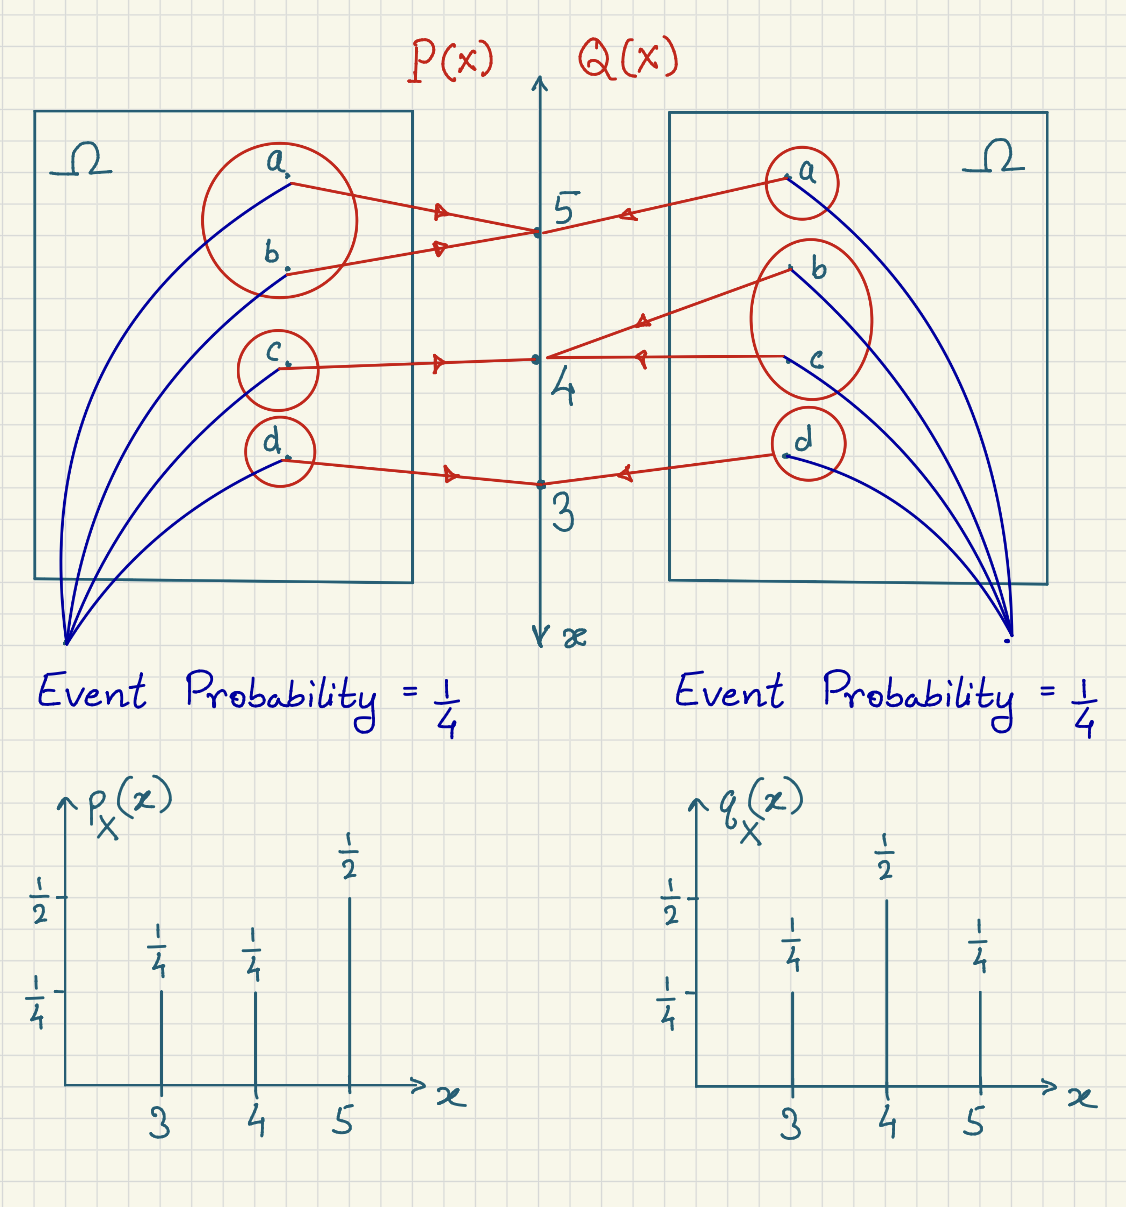
\includegraphics[width=0.75\textwidth]{EntropyExample1.png}
    \caption{Cross-entropy case 1, different distributions $P$ and $Q$.}
    \label{fig:SameSpan}
\end{figure}

For case 1 in \ref{fig:SameSpan}, the cross-entropy is
\begin{align}
    H(P, Q) = -(\frac{1}{4}\,log(\frac{1}{4}) + \frac{1}{4}\, log(\frac{1}{2}) + \frac{1}{2}\,log(\frac{1}{4}))
\end{align}

\begin{figure}[ht]
    \centering
    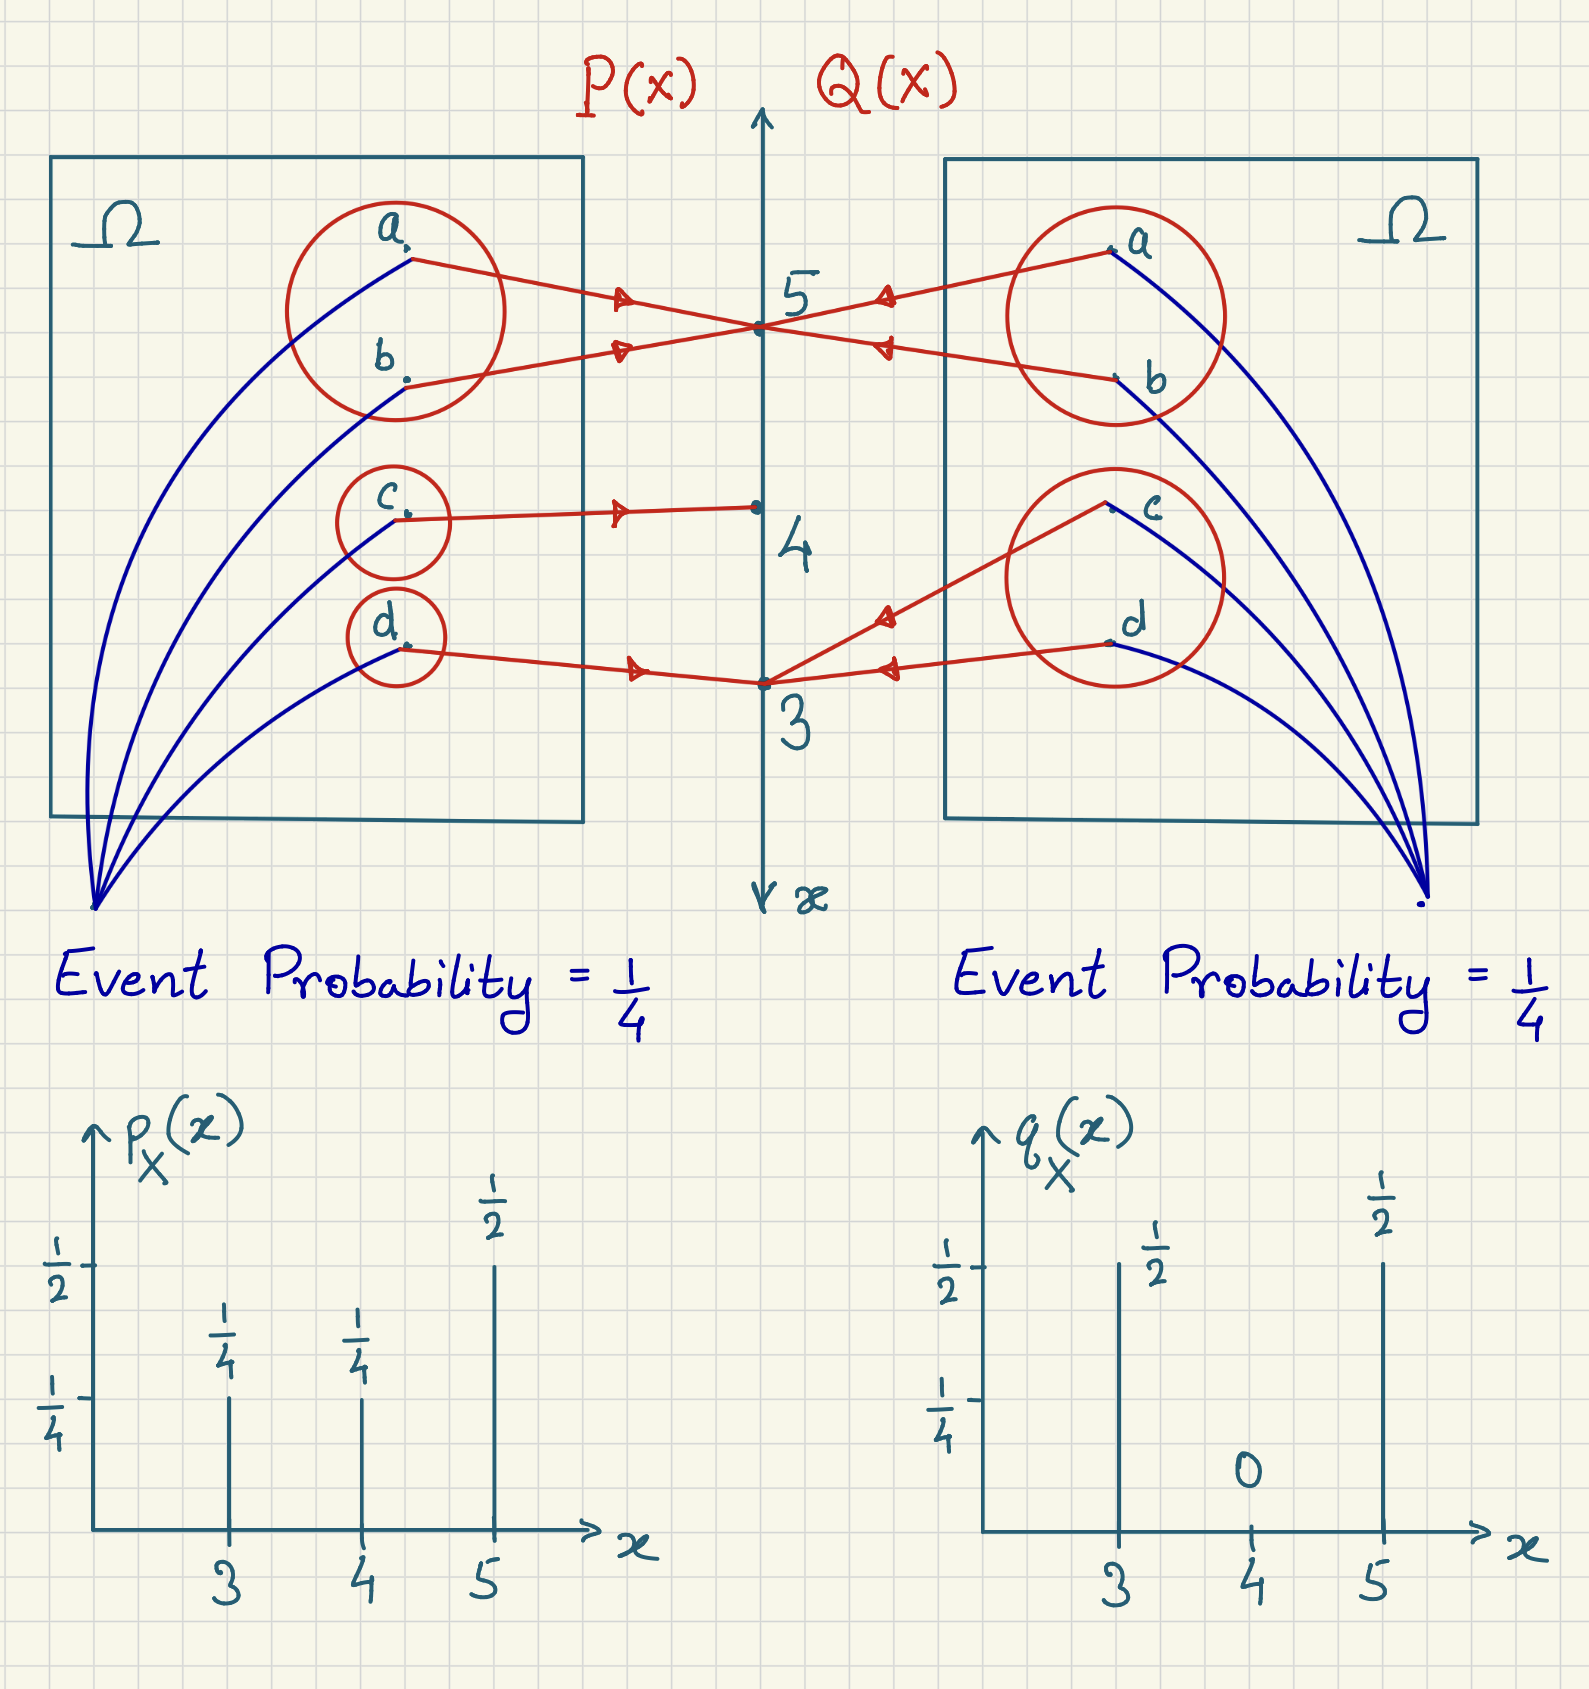
\includegraphics[width=0.75\textwidth]{EntropyExample2.png}
    \caption{Cross-entropy case 2, $Q$ has different set of outcomes.}
    \label{fig:DiffSpan}
\end{figure}

For case 2 in \ref{fig:DiffSpan}, the cross-entropy is
\begin{align}
    H(P, Q) = -(\frac{1}{4}\,log(\frac{1}{2}) + \frac{1}{4}\, log(0) + \frac{1}{2}\,log(\frac{1}{2}))
\end{align}
Note that
\begin{align}
    \lim_{p\rightarrow 0^+}(log\,p) = - \infty
\end{align}
so the cross-entropy $\rightarrow \infty$.

\begin{figure}[ht]
    \centering
    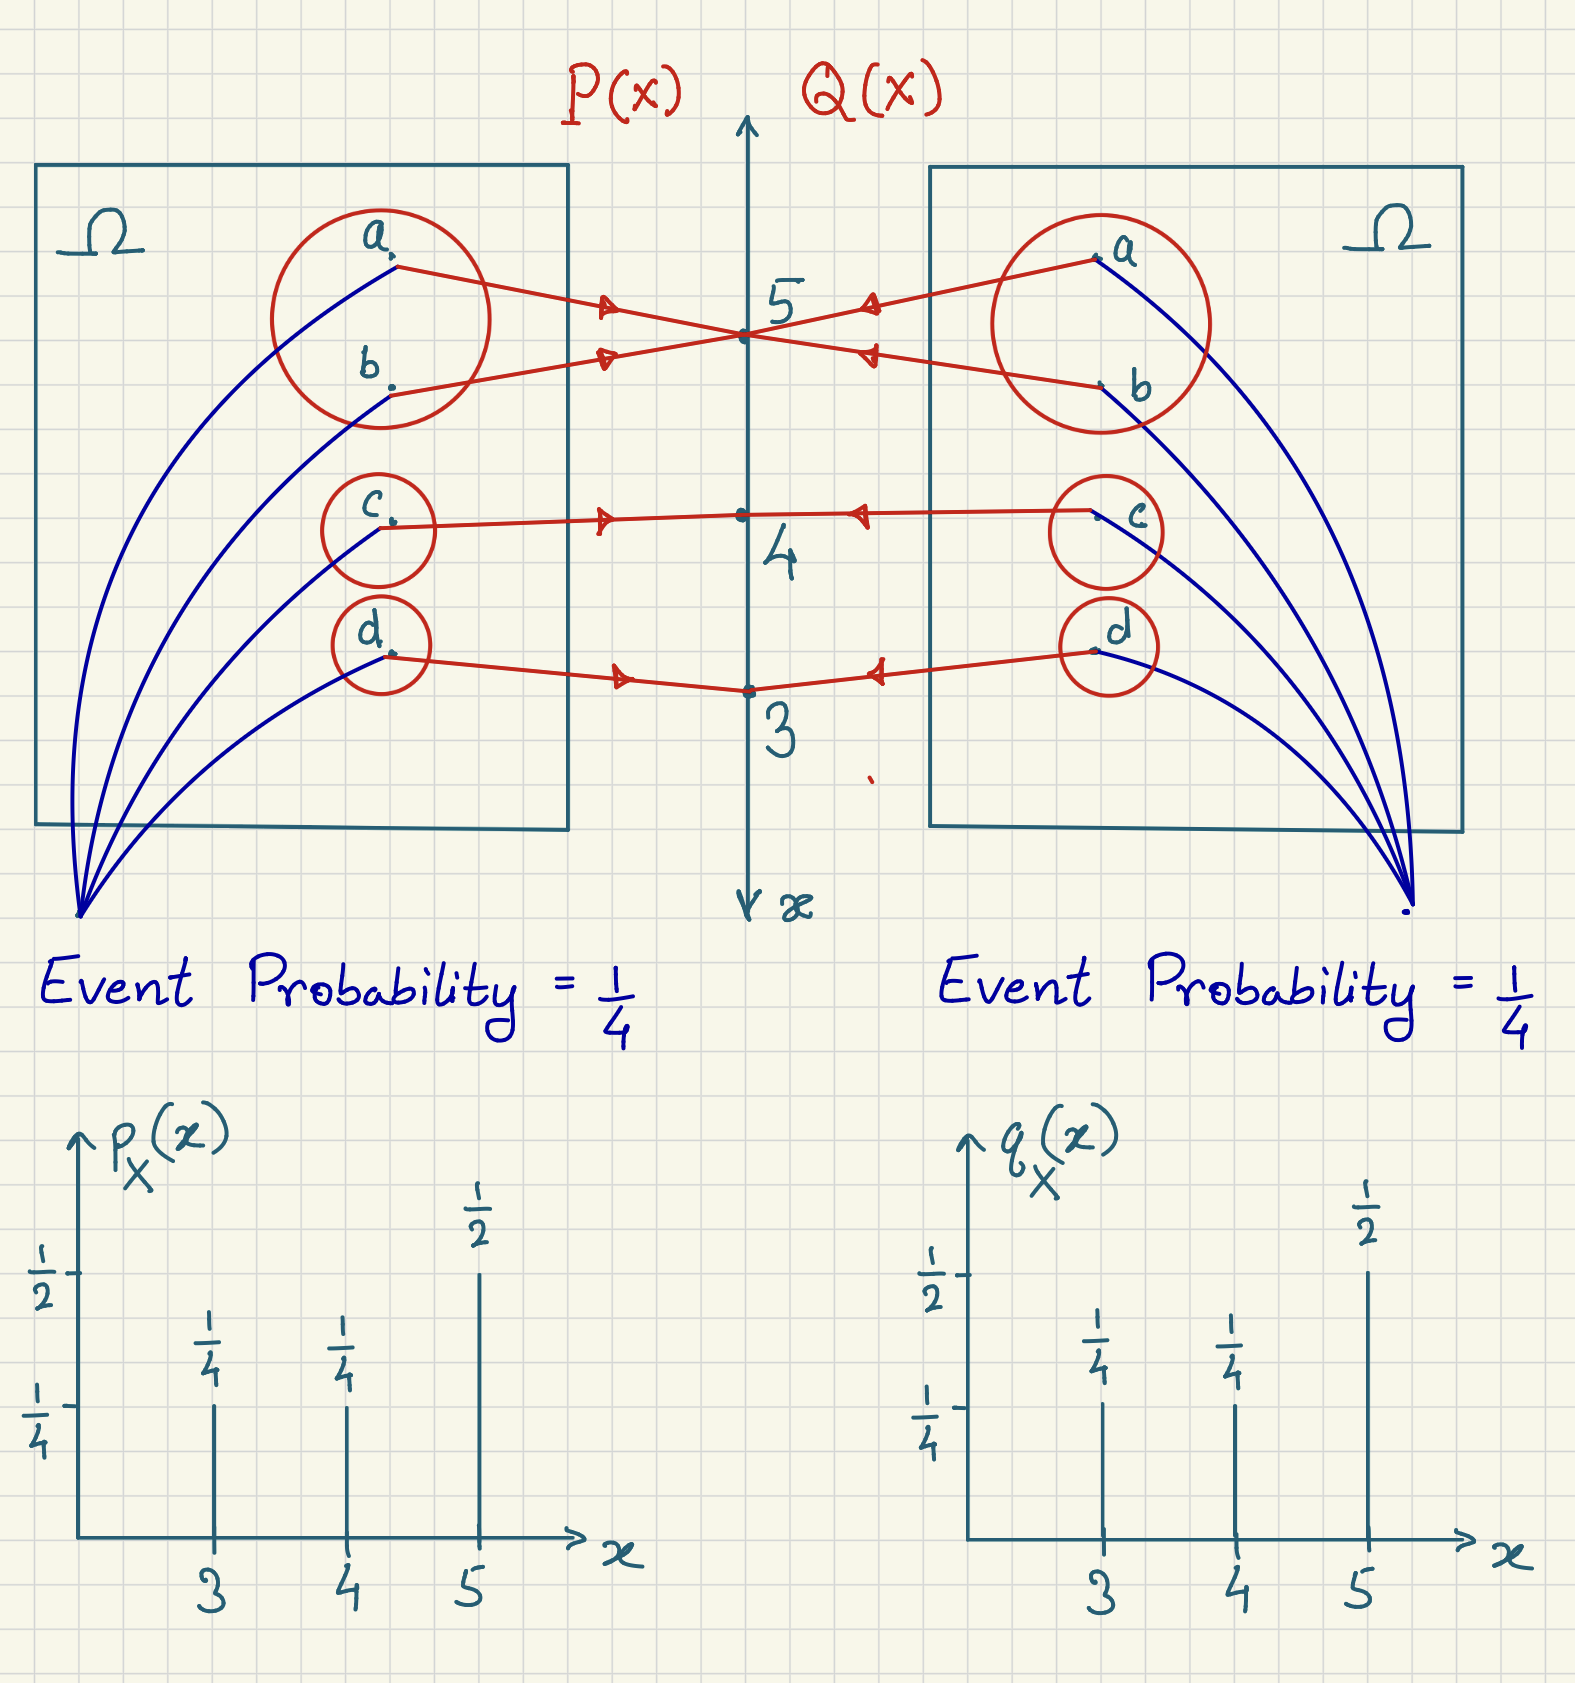
\includegraphics[width=0.75\textwidth]{EntropyExample3.png}
    \caption{Cross-entropy case 3, $P$ and $Q$ identical.}
    \label{fig:SameDist}
\end{figure}

For case 3 in \ref{fig:SameDist}, the cross-entropy is
\begin{align}
    H(P, Q) = -(\frac{1}{4}\,log(\frac{1}{4}) + \frac{1}{4}\, log(\frac{1}{4}) + \frac{1}{2}\,log(\frac{1}{2}))
\end{align}

So cross-entropy measures how well the distribution $Q$ aligns with distribution $P$. If $Q$ assigns low probability to outcomes that are likely under $P$, cross-entropy will increase. Note that we cannot however say that cross-entropy measures deviation of $Q$ from $P$; for that, we have something called KL divergence (mentioned here only for the sake of completeness).

Also note that in all the three examples above, the probability distributions $P$ and $Q$ are known a priori.

In statistics, cross-entropy can be used to measure how well a model's predicted probability distribution matches the true distribution. Let's say we have a model $Q$ to predict the class performance on an exam, with values:

\begin{align}
    q(pass) = 0.75\\[10pt]
    q(fail) = 0.25
\end{align}
Now suppose we have the true class performance for two exams, Biology and Calculus, with values:

Biology
\begin{align}
    p_1(pass) = 0.8\\[10pt]
    p_1(fail) = 0.2
\end{align}

Calculus
\begin{align}
    p_2(pass) = 0.6\\[10pt]
    p_2(fail) = 0.4
\end{align}

Using cross-entropy to quantify the model performance for Biology (model with respect to Biology):
\begin{align}
    H(P_1, Q) & = - \mathbb{E}_{X\sim P_1}[log(q(X))]\\[10pt]
    & = -\sum_i p_1(x_i) \, log(q(x_i))\\
    & = -[p_1(pass)\,log(q(pass)) + p_1(fail)\,log(q(fail))]\\[10pt]
    & = -[0.8\,log(0.75) + 0.2\,log(0.25)]\\[10pt]
    & \approx 0.507\,nats
\end{align}
Model performance for Calculus:
\begin{align}
    H(P_2, Q) & = - \mathbb{E}_{X\sim P_2}[log(q(X))]\\[10pt]
    & = -\sum_i p_2(x_i) \, log(q(x_i))\\
    & = -[p_2(pass)\,log(q(pass)) + p_2(fail)\,log(q(fail))]\\[10pt]
    & = -[0.6\,log(0.75) + 0.4\,log(0.25)]\\[10pt]
    & \approx 0.727\,nats
\end{align}

So the model aligns more closely with the true Biology distribution than the true Calculus distribution.

Also, the average cross-entropy is
\begin{align}
    -\frac{1}{2} [\mathbb{E}_{X\sim P_1}[log(q(X))] + \mathbb{E}_{X\sim P_2}[log(q(X))]] \approx 0.617\,nats
\end{align}

\subsection{Population cross-entropy}
In machine learning and optimization, cross-entropy is defined as expectation over the \textbf{population} and is called \textbf{population cross-entropy}
\begin{align}
    = -\mathbb{E}_{X\sim P}[log(q(X))]]
\end{align}
If $P$ and $Q$ are known, it can be calculated before any value of $X$ is observed - which is never the case in machine learning. To understand this, consider the scenario in supervised learning. Here, each example is usually a pair $(x, y)$:

\hspace{40pt} x: input such as an image, a sentence

\hspace{40pt} y: label such as "cat", "positive sentiment"

There is a true underlying population distribution given by
\begin{align}
    P_{data}(x, y)
\end{align}
and the population cross-entropy gives us a measure to quantify the accuracy of model assigned probabilities. It is like asking if the real world kept producing examples forever, how well would this model assign probabilities to the correct labels on average? 

Computed as a loss given by 
\begin{align}
    L(\theta) = \mathbb{E}_{(x, y) \sim P_{data}} [-log(q_{\theta} (y\,|\,x)]
\end{align}

where $q_{\theta}(y\,|\,x)$ is the model's predicted probability for label $y$ given $x$, and $\theta$ represents model parameters.

We usually do not have this distribution $P_{data}$, so we only observe a finite number of examples (like we would observe arriving buses at a bus stop in an effort to compute inter-arrival time):
\begin{align}
    (x^1, y^1), (x^2, y^2), ... , (x^n, y^n)
\end{align}
The loss computed using this sample, called \textbf{empirical cross-entropy}, is
\begin{align}
    \hat{L}(\theta) = \frac{1}{n} \sum_{j=1}^{n} -log(q_{\theta} (y^j | x^j))
\end{align}
assuming uniform distribution.

Training the model then means choosing a starting model distribution $Q_{\theta}$ and updating over many samples to a $Q$ that (hopefully) best approximates $P$. We do this by a process called ``learning'' in which we minimize $\hat{L}(\theta)$ by updating $\theta$ using gradient descent. Note that gradient descent does not guarantee that we arrive at any such $\theta$.

\section{Gradient of population cross-entropy loss}
Consider the neural network given in figure \ref{fig:NeuralNetwork}, with ReLU activation functions (denoted by f) on all neurons and softmax activation function in the output layer.

\begin{figure}[ht]
    \centering
    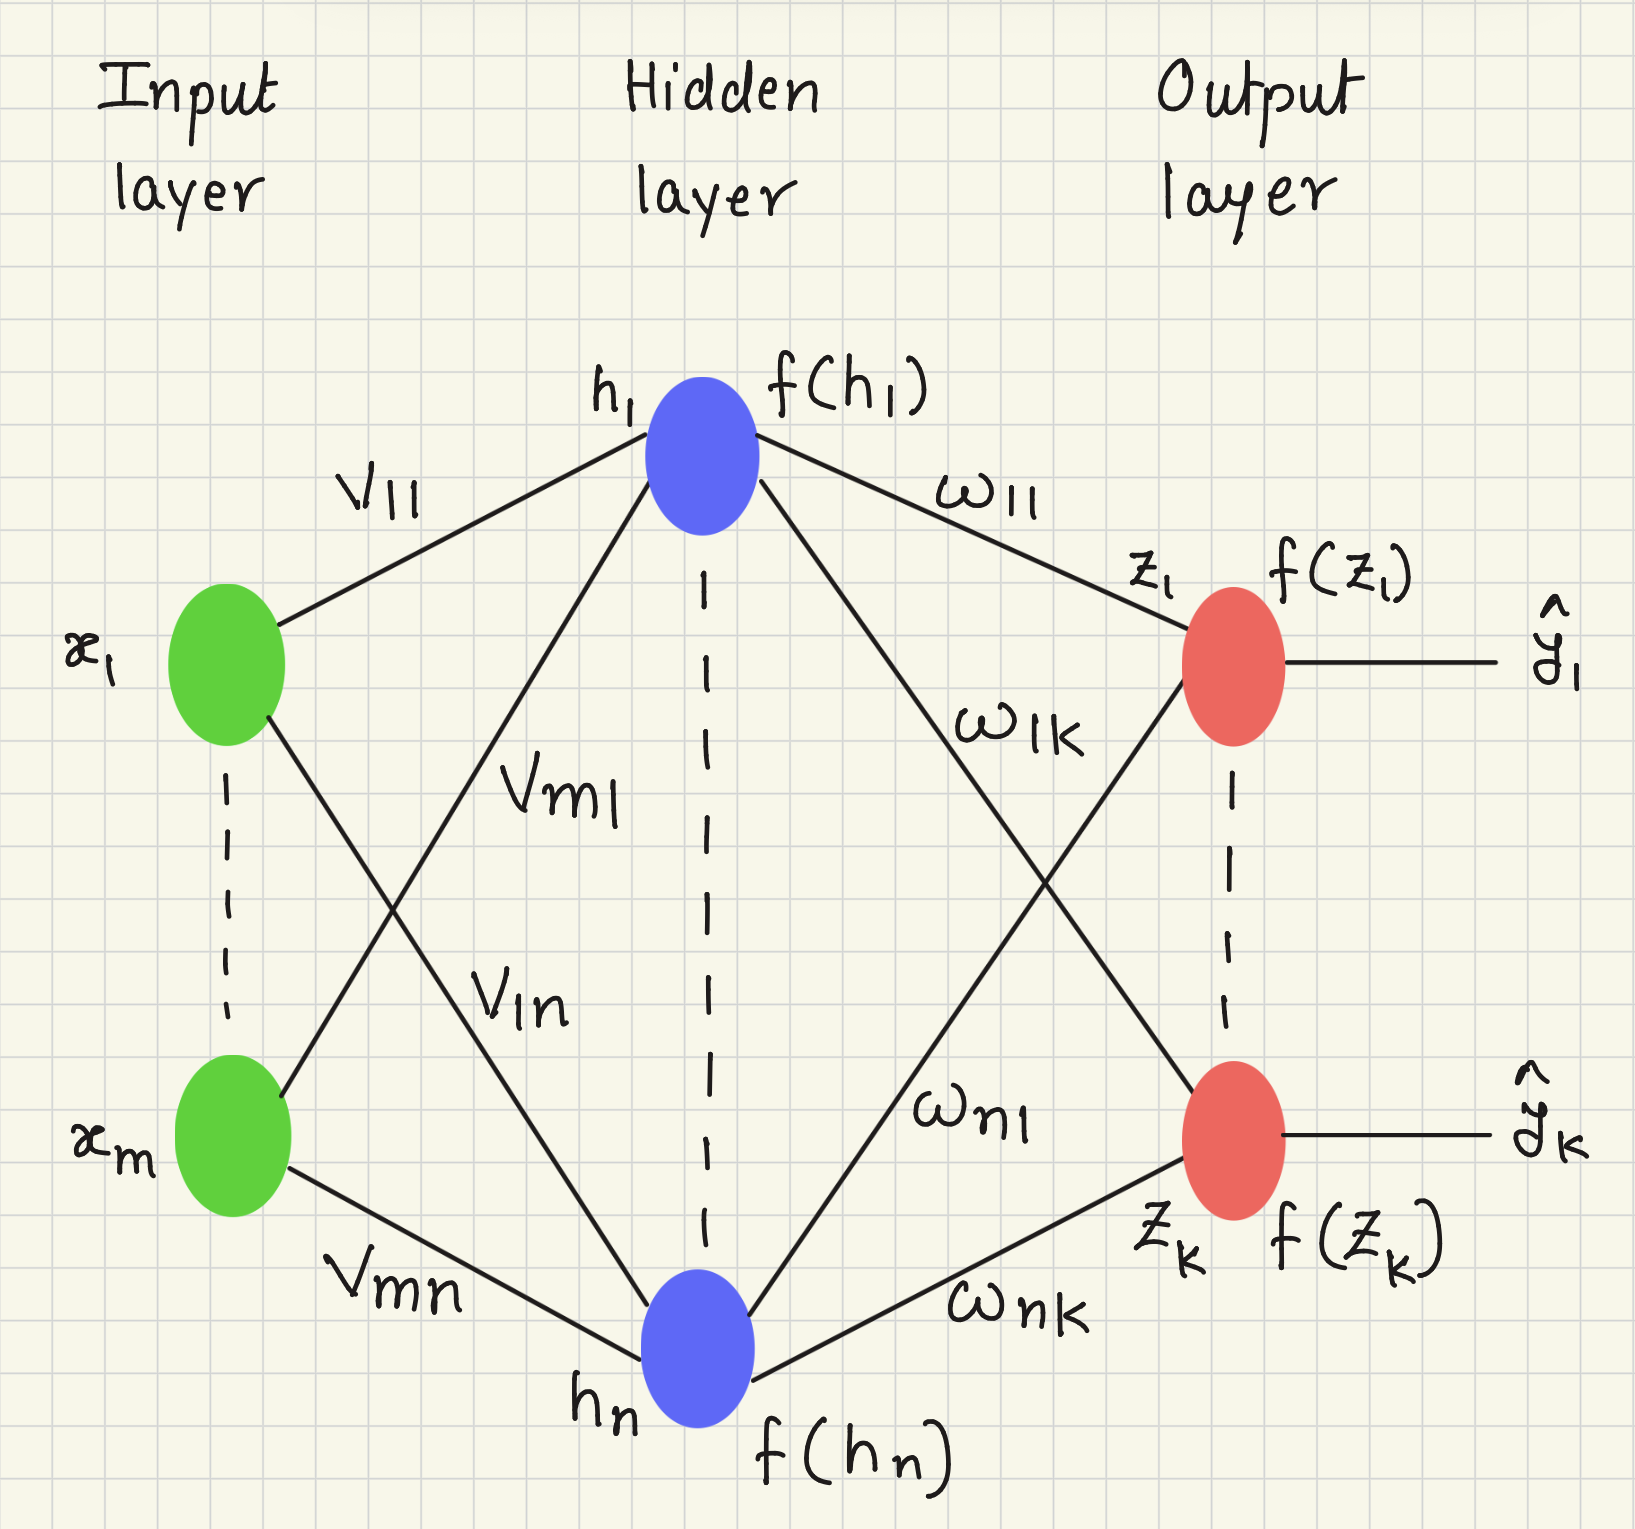
\includegraphics[width=0.75\textwidth]{EntropyNeuralNetwork.png}
    \caption{A simple neural network.}
    \label{fig:NeuralNetwork}
\end{figure}

Given an input $[x_1, x_2, ..., x_m]^T$, the hidden units in the network are activated in stages as described by the following system of equations:

\[ \left(
\begin{array}{cccc}
v_{11} & v_{21} & \ldots & v_{m1} \\
v_{12} & v_{22} & \ldots & v_{m2} \\
\vdots & \vdots & \vdots & \vdots \\
v_{1n} & v_{2n} & \ldots & v_{mn}
\end{array}
\right) 
\left(
\begin{array}{cccc}
x_{1} \\
x_{2} \\
\vdots \\
x_{m}
\end{array}
\right)
+ 
\left(
\begin{array}{cccc}
v_{01} \\
v_{02} \\
\vdots \\
v_{0n}
\end{array}
\right)
=
\left(
\begin{array}{cccc}
h_{1} \\
h_{2} \\
\vdots \\
h_{n}
\end{array}
\right)
\]

\[
\begin{array}{ccc}
f(h_1) & = & max\{h_1, 0\} \\
f(h_2) & = & max\{h_2, 0\} \\
\vdots & & \vdots \\
f(h_n) & = & max\{h_n, 0\}
\end{array}
\]

\begin{align}
    h_i = v_{0i} + \sum_{j=1}^m {v_{ji}x_j},
    \hspace{30pt} 1 \leq i \leq n
\end{align}

\[ \left(
\begin{array}{cccc}
w_{11} & w_{21} & \ldots & w_{n1} \\
w_{12} & w_{22} & \ldots & w_{n2} \\
\vdots & \vdots & \vdots & \vdots \\
w_{1k} & w_{2k} & \ldots & w_{nk}
\end{array}
\right)
\left(
\begin{array}{cccc}
f(h_1) \\
f(h_2) \\
\vdots \\
f(h_n)
\end{array}
\right)
+ 
\left(
\begin{array}{cccc}
w_{01} \\
w_{02} \\
\vdots \\
w_{0k}
\end{array}
\right)
=
\left(
\begin{array}{cccc}
z_{1} \\
z_{2} \\
\vdots \\
z_{k}
\end{array}
\right)
\]

\[
\begin{array}{ccc}
f(z_1) & = & max\{z_1, 0\} \\
f(z_2) & = & max\{z_2, 0\} \\
\vdots & & \vdots \\
f(z_k) & = & max\{z_k, 0\}
\end{array}
\]

\begin{align}
    z_i = w_{0i} + \sum_{j=1}^n {w_{ji}\,f(h_j)},
    \hspace{30pt} 1 \leq i \leq k.
\end{align}

The final output of the network is obtained by applying the softmax function to the last hidden layer,

\[
\hat{y} = 
\left(
\begin{array}{c}
\hat{y_1} \\
\hat{y_2} \\
\vdots \\
\hat{y_k}
\end{array}
\right)
\hspace{10pt} where \hspace{10pt}
\hat{y_i} = \frac{e^{f(z_i)}}{\sum_{j=1}^k{e^{f(z_j)}}}
\hspace{40pt} 1 \leq i \leq k.
\]

Assume that $V$ is a constant matrix and also, for simplicity, assume that $f(z_i) = z_i$ and $f(h_i) = h_i$ to stay focused on computing gradient of cross-entropy without bringing in ReLU.

Then cross-entropy loss for a single example is
\begin{align}
    L(\theta) = L(W) = - \sum_{i=1}^k {y_i \, log(\hat{y_i})}.
\end{align}
and the gradient of $L$ with reference to $W$ is
\[ \nabla_W L = \left(
\begin{array}{cccc}
\frac{\partial L}{w_{11}} & \frac{\partial L}{w_{21}} & \ldots & \frac{\partial L}{w_{n1}} \\[10pt]
\frac{\partial L}{w_{12}} & \frac{\partial L}{w_{22}} & \ldots & \frac{\partial L}{w_{n2}} \\[10pt]
\vdots & \vdots & \vdots & \vdots \\[10pt]
\frac{\partial L}{w_{1k}} & \frac{\partial L}{w_{2k}} & \ldots & \frac{\partial L}{w_{nk}}
\end{array}
\right) \]
Now consider
\begin{align}
    \frac{\partial L}{\partial w_{21}} & = \frac{\partial}{\partial w_{21}} \left[- \sum_{i=1}^k y_i \, log(\hat{y_i}) \right] \\
    & = \sum_{i=1}^k - y_i \, \frac{\partial \, log(\hat{y_i})}{\partial \hat{y_i}} \, \frac{\partial \hat{y_i}}{\partial w_{21}} \\
    & = \sum_{i=1}^k - y_i \, \frac{1}{\hat{y_i}} \, \frac{\partial \hat{y_i}}{\partial z_1} \, \frac{\partial z_1}{\partial w_{21}}
\end{align}
Now,
\begin{align}
    \frac{\partial z_1}{\partial w_{21}} & = \frac{\partial} {\partial w_{21}} \, \left( w_{01} + \sum_{j=1}^n w_{j1} h_j \right) \\[10pt]
    & = h_2
\end{align}
and we have two cases for $\frac{\partial \hat{y_i}}{\partial z_1}$.

Case 1: $i = 1$

\begin{align}
    \frac{\partial \hat{y_1}}{\partial z_1} & = \frac{\partial}{\partial z_1} \left( \frac{e^{z_1}}{\sum_{j=1}^k e^{z_j}} \right) \\[10pt]
    & = \frac{e^{z_1} \, \sum_{j=1}^k (e^{z_j}) - e^{z_1} \, e^{z_1}}{(\sum_{j=1}^k (e^{z_j}))^2} \\[10pt]
    & = \left( \frac{e^{z_1}}{\sum_{j=1}^k (e^{z_j})}\right) - \left( \frac{e^{z_1}}{\sum_{j=1}^k (e^{z_j})}\right)^2\\[10pt]
    & = \hat{y_1} - (\hat{y_1})^2
\end{align}

Case 2: $i \neq 1$
\begin{align}
    \frac{\partial \hat{y_i}}{\partial z_1} & = \frac{\partial}{\partial z_1} \left( \frac{e^{z_i}}{\sum_{j=1}^k e^{z_j}} \right) \\[10pt]
    & = \frac{0 - e^{z_i} \, e^{z_1}}{(\sum_{j=1}^k (e^{z_j}))^2} \\[10pt]
    & = -\hat{y_i}\, \hat{y_1}
\end{align}

Now plugging back into the equation for $\frac{\partial L}{\partial w_{21}}$
\begin{align}
    \frac{\partial L}{\partial w_{21}} & = - ( y_1 (1-\hat{y_1}) - \hat{y_1} \, y_2 - ... - \hat{y_1} \, y_k ) \, h_2 \\[10pt]
    & = - \left( y_1 - \hat{y_1} \, y_1 \, - \hat{y_1} \, y_2 - ... - \hat{y_1} \, y_k \right) \, h_2\\[10pt]
    & = - (y_1 - \hat{y_1}( y_1 + y_2 + ... + y_k )) \, h_2 \\[10pt]
    & = (\hat{y_1} - y_1) \, h_2
\end{align}
since $y_1 + ... + y_k = 1$.

It is easy to see that this generalizes to
\begin{align}
    \frac{\partial L}{\partial w_{ji}} = (\hat{y_i} - y_i) \, h_j
\end{align}
which is nothing but the difference between the predicted and the ground truth probability distributions, scaled by the embeddings. This simplicity makes population cross-entropy along with softmax a popular combination for transformer models.

\end{document}